\documentclass[annual]{acmsiggraph}
\usepackage{wrapfig}
\usepackage{hyperref}
\title{X\texorpdfstring{\textsuperscript{2}}-Toon: An Extended X-Toon Shader}

\author{Robert Wolfe\thanks{e-mail:robert\_wolfe@carleton.ca}\\Spencer Elliott\thanks{e-mail:spencer\_elliott@carleton.ca}}
\pdfauthor{Robert Wolfe, Spencer Elliott}

\keywords{xtoon, image processing, xna}

\begin{document}

\maketitle

\begin{abstract}

X-toon ~\cite{BTM06a} extended classic cel shading.

\end{abstract}

\keywordlist

\copyrightspace

\section{Introduction}
~\cite{BTM06a} extended the classical understanding of how to perform toon shading. A new dimension of tone detail can be used to create a desired level of abstraction. Our approach implements this technique, as well as extends it. We first developed a standard cel shader using ~\cite{CelShadingTut} as a starting point. Using models downloaded from ~\cite{TurboSquid} and (*\textbf{where did we download the dude and axes??}), we used a threshold of the dot product of the lighting vector and the surface normal to produce classic toon shading. An example can be seen in Figure~\ref{fig:toonshade}.

\begin{figure}[h]
	\centering
	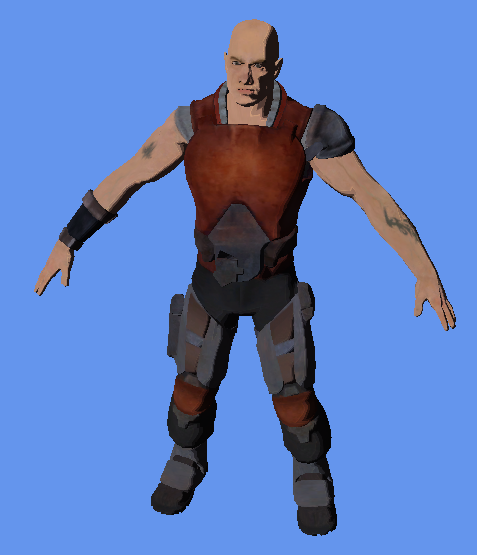
\includegraphics[width=1.5in]{images/classic_cel2}
	\caption{Classic Toon Shading}
	\label{fig:toonshade}
\end{figure}

A brief explanation of X-Toon is described in Section~\ref{sec:tonedetail}, our extensions in Section~\ref{sec:extensions}, and the results in Section~\ref{sec:results}. Discussion and future work are described in Section~\ref{sec:discussion} and finally the conclusion in Section~\ref{sec:conclusion}.

To make our program more interactive, we developed a GUI using the XNA GUI framework from ~\cite{Ruminate}. The controls allows the user to modify the parameters and enabled/disable features.

\section{Tone Detail}
\label{sec:tonedetail}
\begin{wrapfigure}{r}{0.1\textwidth}
  \vspace{-20pt}
  \begin{center}
    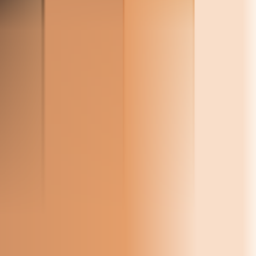
\includegraphics[width=0.1\textwidth]{images/xtoon_skin}
  \end{center}
  \caption{2D Texture.}
  \vspace{-10pt}
  \label{fig:2dtexture}
\end{wrapfigure}
We extend the concept of a regular toon shader by adding a second dimension to the texture. While the x-axis remains as $N\cdot L$, where {\it{N}} is the surface normal and {\it{L}} is the light direction, the y-axis represents the level of detail. The higher up on the axis, the less detail is used. Conversely, the lower the y-axis value, the more detail. An example of a 2D texture used in this application can be seen in Figure~\ref{fig:2dtexture} (note the y-axis increases downward).

The method of computing the y-axis depends on an {\it{attribute map.}} The chosen attribute changes the level of detail, depending on its value. The original paper provided two possible attribute maps: distance and orientation. This paper deals exclusively with the distance attribute mapping. We provide an alternative mapping involving the angle between the camera {\it{look at}} vector and surface normal. 

In addition to providing an alternate attribute mapping, we also developed a new method for determining the amount of shading on a model. This method involves calculating direction vectors to each light from each vertex. The resulting vector can then be used to calculate the final shading amount.

\subsection{Distance}
As in the original X-Toon paper, one attribute map uses the focal distance of the vertex to the camera. The larger this distance, the less detail will be used, abstracting the model. The smaller this distance, the more detail used. Nothing was changed from the original paper. An example result can be seen in Figure~\ref{fig:distanceResult}, using a transparent texture map (see Section~\ref{sec:transparency}).

\begin{figure}[h]
	\centering
	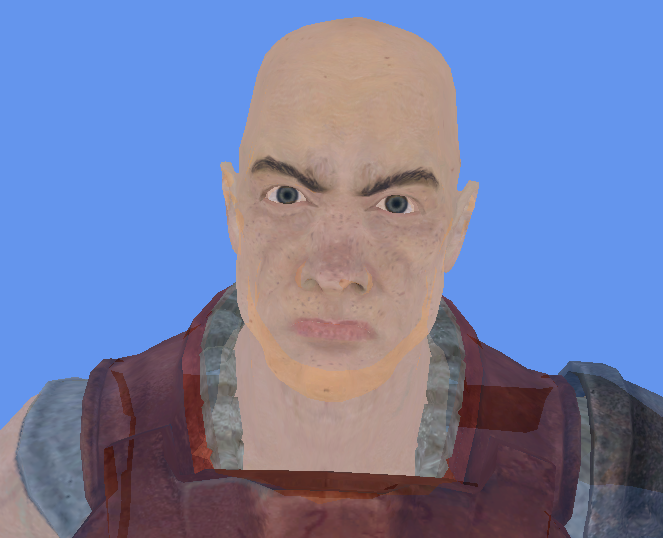
\includegraphics[width=2.5in]{images/distance_result}
	\caption{Parts of the model that are farther away are more transparent than closer areas.}
	\label{fig:distanceResult}
\end{figure}

\subsection{Angle}
We introduce a new attribute map based on the angles of the {\it{look at}} of the camera and the surface normal. The look at vector is the direction that the camera is pointed. The angle between the two vectors is calculated using Equation~\ref{eqn:angle}, which is derived from the formula for dot product.

\begin{equation}
\label{eqn:angle}
a = \cos^{-1}{(-LookAt \cdot Normal / |LookAt||Normal|)}
\end{equation}

The negative of the look at vector is used because it is pointed towards the surface (see Figure~\ref{fig:angle}). This value indicates what surfaces the camera is directly pointed at. The amount of detail used decreases as the angle between the look at vector and the surface normal approaches $180^\circ$, or when the surface is completely pointed away from the camera (or vice versa). As the angle approaches 0, more detail is used. An example result of this attribute map can be seen in Figure~\ref{fig:angleResult}.

\begin{figure}[h]
	\centering
	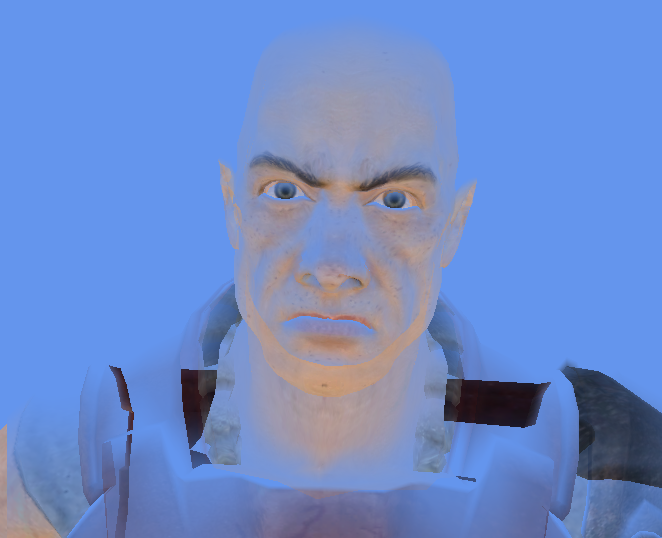
\includegraphics[width=2.5in]{images/angle_result}
	\caption{An example result of the angle attribute map/}
	\label{fig:angleResult}
\end{figure}

\begin{figure}[h]
	\centering
	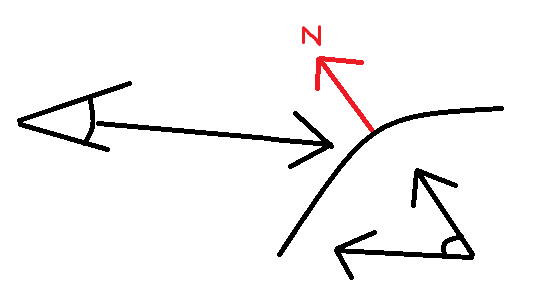
\includegraphics[width=1.5in]{images/angle}
	\caption{Diagram of the angle calculation using the camera (left)'s look at vector and the surface normal (right). The angle difference is calculated (bottom right) using Equation~\ref{eqn:angle}.}
	\label{fig:angle}
\end{figure}

\subsection{Light Direction}
We developed a new method to determine the x-axis value based on the lighting of a scene. The direction to each light in the scene is determined for every vertex. These directions would then be summed and a resulting direction vector would be created. The direction vector is normalized and the final detail is calculated using the same equation for determining the 

\begin{figure}[h]
	\centering
	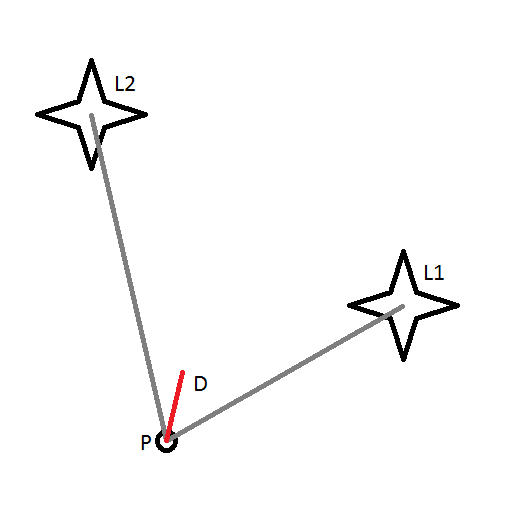
\includegraphics[width=1.5in]{images/light_detail}
	\caption{A diagram explaining the light direction attribute map.}
	\label{fig:lightDirection}
\end{figure}

\begin{figure}[h]
	\centering
	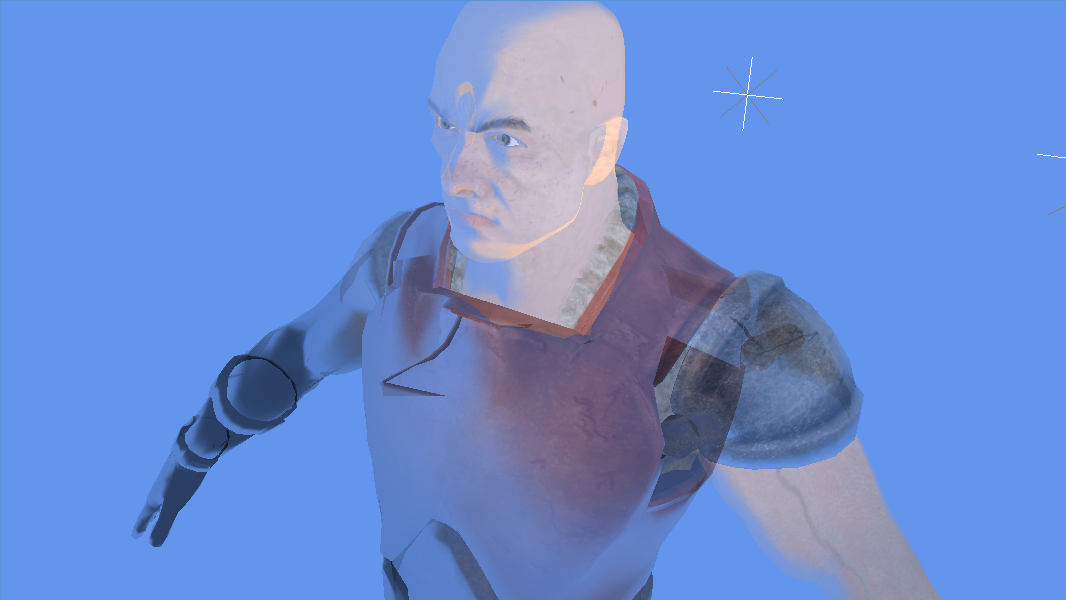
\includegraphics[width=3.0in]{images/light_directions}
	\caption{An example result of using the light direction attribute map.}
	\label{fig:lightDirectionResult}
\end{figure}

\section{Extensions to original X-Toon shader}
\label{sec:extensions}
We have extended the original shader offered in the X-Toon paper to increase the usability for various new effects. The first extension involves using colours from the original model's textures when calculating the final detail. The second extension allows for the use of transparency in both the tone texture and original model's textures to create 

\subsection{Texture blending}
We have added the ability to blend textures from a model into the calculation of the shading and tone detail. This technique gives artists the ability to retain the original look of the model while also applying the X-Toon effects. To achieve this effect, our shader first takes the pixel sample from the original texture. The shading and detail are determined using the calculations explained in previous sections and the final tone detail pixel is kept. To mix the colours of the original texture and the tone detail pixel, a simple multiplication of the {\it{RGB}} channels is performed. The resulting pixel is a blend of the original texture pixel and the sampled tone detail texture. Figure~\ref{fig:texturing} shows an example of a model with and without texture blending.

\begin{figure}[h]
	\centering
	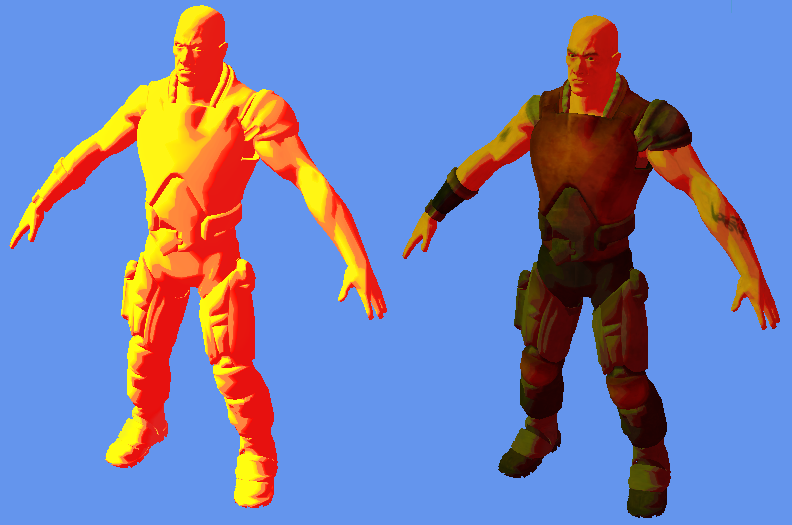
\includegraphics[width=3.0in]{images/textures}
	\caption{A model without and with original textures applied, respectively}
	\label{fig:texturing}
\end{figure}

\subsection{Texture transparency}
\label{sec:transparency}

\begin{figure}[h]
	\centering
	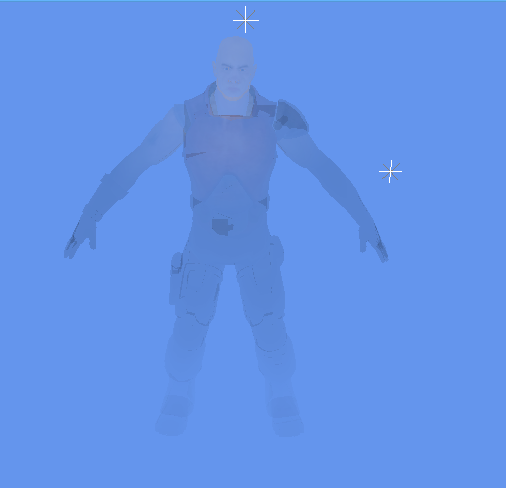
\includegraphics[width=2.5in]{images/transparency}
	\caption{Transparency affecting output}
	\label{fig:transparency}
\end{figure}

\section{Results}
\label{sec:results}
Some results are ablkjalskdjalskdjasd.

\begin{figure}[h]
	\centering
	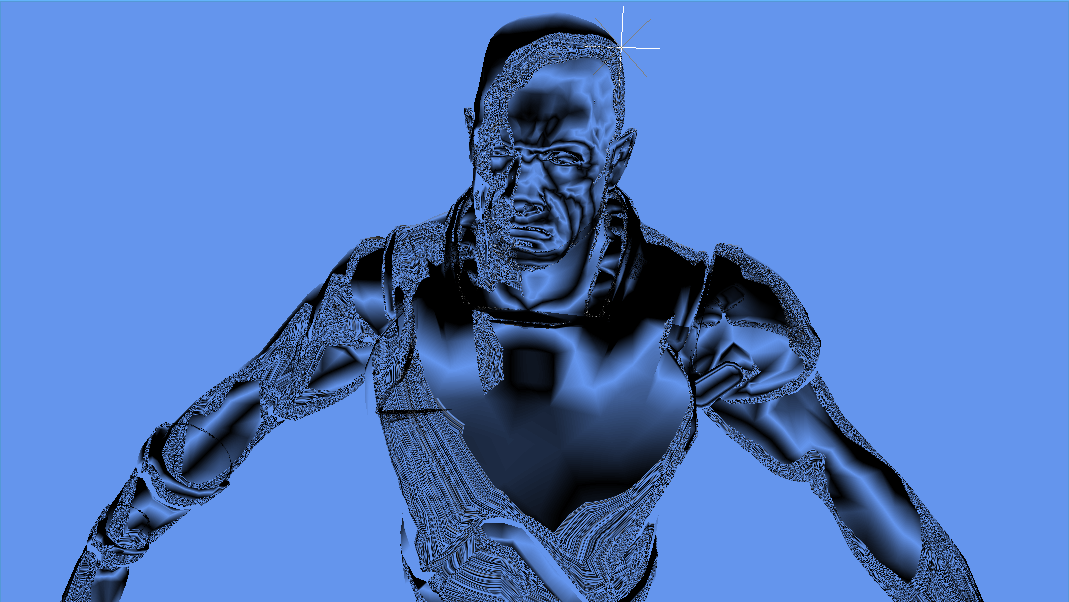
\includegraphics[width=5.5in]{images/hologram}
	\caption{Hologram result}
	\label{fig:hologram}
\end{figure}

\begin{figure}[p]
	\centering
	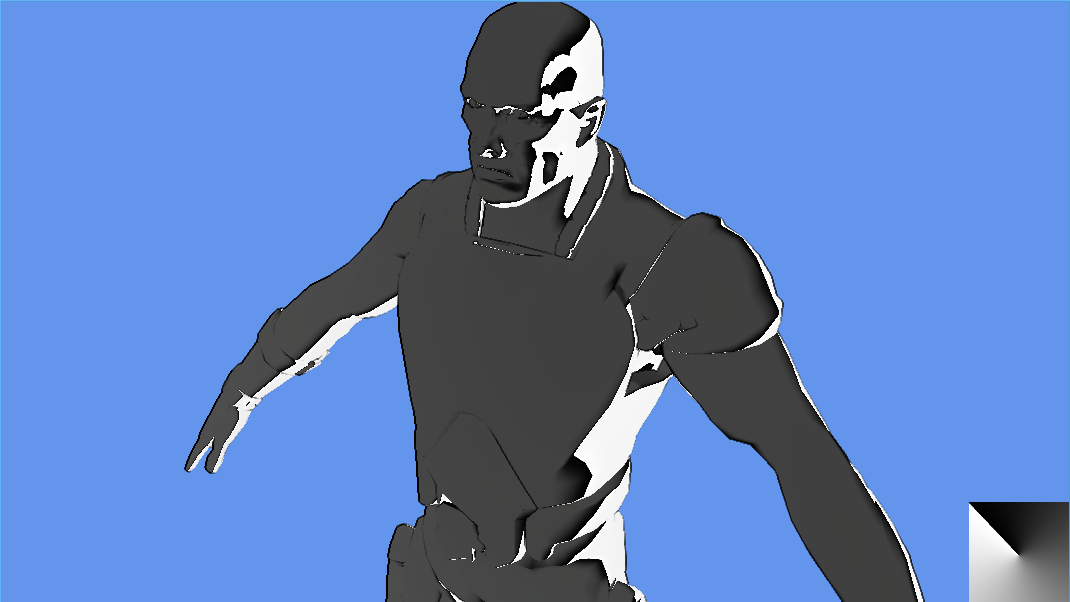
\includegraphics[width=5.5in]{images/inverse_lighting}
	\caption{Inverse Lighting result}
	\label{fig:inverseLighting}
\end{figure}

\begin{figure}[p]
	\centering
	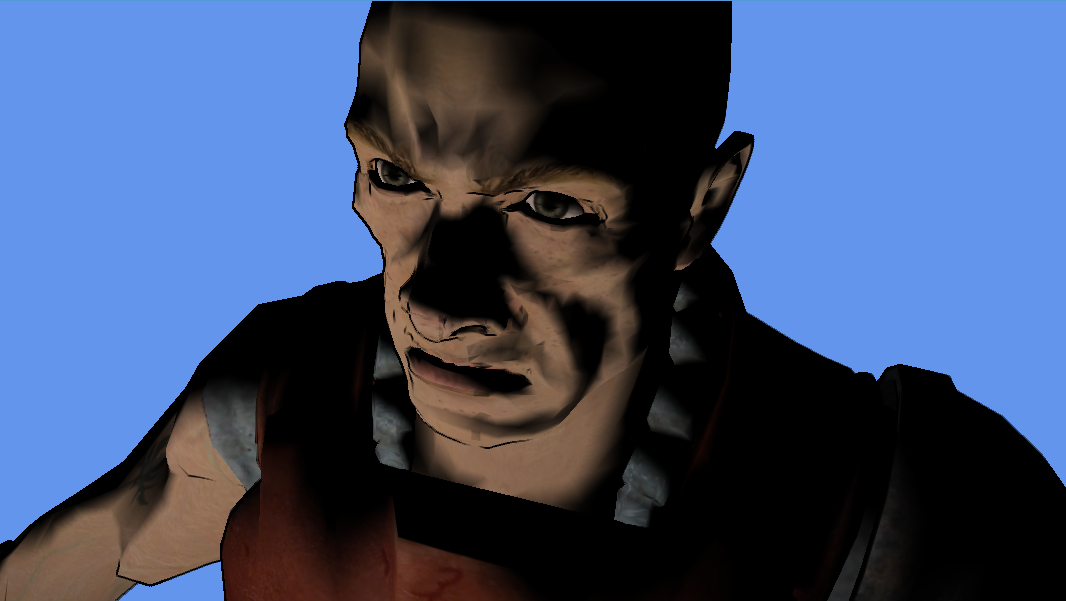
\includegraphics[width=5.5in]{images/lighting}
	\caption{Lighting result}
	\label{fig:lightingResult}
\end{figure}

\begin{figure}[p]
	\centering
	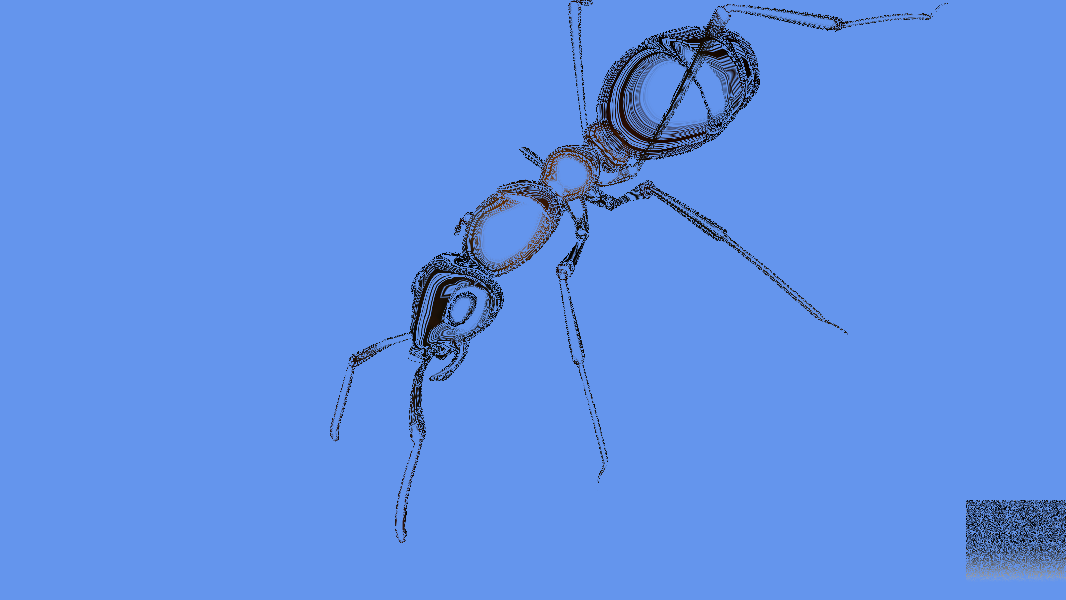
\includegraphics[width=5.5in]{images/stipple-hatch-result1}
	\caption{Stipple/hatching result}
	\label{fig:stippleHatch1}
\end{figure}

\begin{figure}[p]
	\centering
	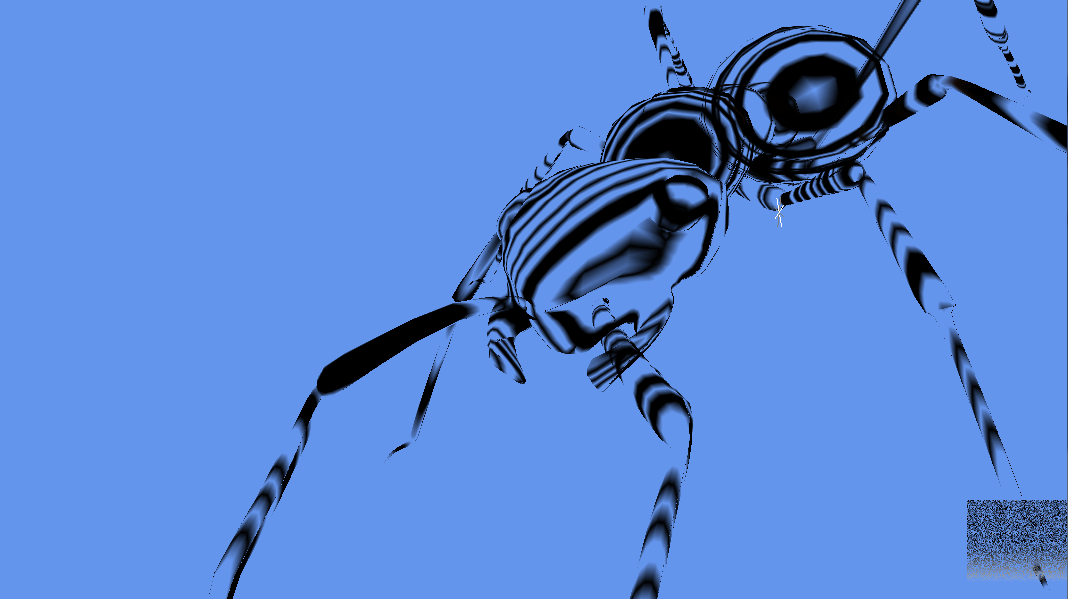
\includegraphics[width=5.5in]{images/stipple-hatch-result2}
	\caption{Stipple/hatching result}
	\label{fig:stippleHatch2}
\end{figure}

\begin{figure}[p]
  \centering
  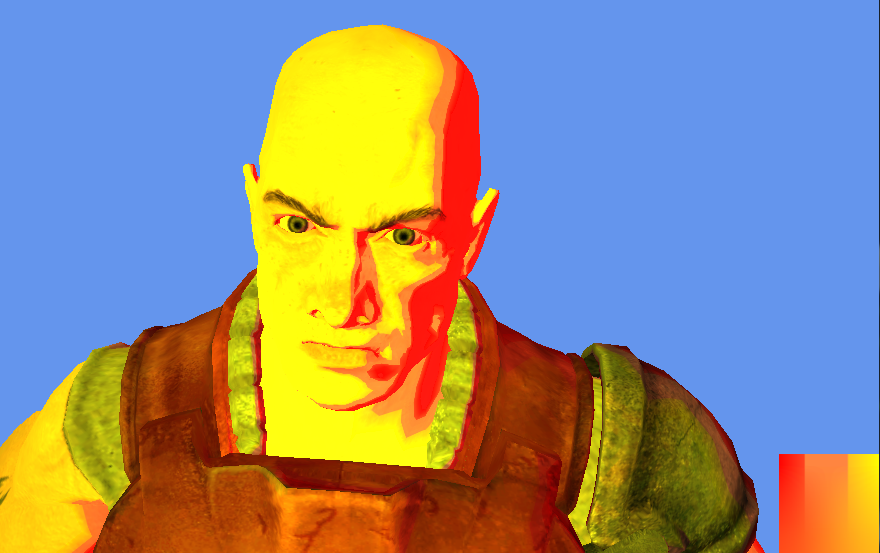
\includegraphics[width=5.5in]{images/test}
  \caption{Sample illustration.}
\end{figure}


\section{Discussion and Future Work}
\label{sec:discussion}

\subsection{Alpha blending correction}


\section{Conclusion}
\label{sec:conclusion}


\bibliographystyle{acmsiggraph}
\bibliography{paper}
\end{document}
